\documentclass[12pt]{article}
\usepackage[utf8]{inputenc}

\usepackage{enumitem}
\usepackage[margin=2cm]{geometry}

\usepackage{amsmath, amsfonts, amssymb}
\usepackage{graphicx}
\usepackage{tikz}
\usepackage{pgfplots}
\usepackage{multicol}

\usepackage{comment}
\usepackage{url}
\usepackage{calc}
\usepackage{subcaption}
\usepackage{circledsteps}
\usepackage{wrapfig}
\usepackage{array}

\setlength\parindent{0pt}

\usepackage{fancyhdr}
\pagestyle{fancy}
\fancyhf{}
\renewcommand{\headrulewidth}{2pt}
\renewcommand{\footrulewidth}{0pt}
\rfoot{\thepage}
\lhead{\textsc{Math} 244}
\chead{\textsc{Homework 12}}
\rhead{Fall 2023}

\pgfplotsset{compat=1.16}

% MATH commands
\newcommand{\ga}{\left\langle}
\newcommand{\da}{\right\rangle}
\newcommand{\oa}{\left\lbrace}
\newcommand{\fa}{\right\rbrace}
\newcommand{\oc}{\left[}
\newcommand{\fc}{\right]}
\newcommand{\op}{\left(}
\newcommand{\fp}{\right)}

\newcommand{\bi}{\mathbf{i}}
\newcommand{\bj}{\mathbf{j}}
\newcommand{\bk}{\mathbf{k}}
\newcommand{\bF}{\mathbf{F}}

\newcommand{\ra}{\rightarrow}
\newcommand{\Ra}{\Rightarrow}

\newcommand{\sech}{\mathrm{sech}\,}
\newcommand{\csch}{\mathrm{csch}\,}
\newcommand{\curl}{\mathrm{curl}\,}
\newcommand{\dive}{\mathrm{div}\,}

\newcommand{\ve}{\varepsilon}
\newcommand{\spc}{\vspace*{0.5cm}}

\DeclareMathOperator{\Ran}{Ran}
\DeclareMathOperator{\Dom}{Dom}

\newcommand{\exo}[3]{\noindent\textcolor{red}{\fbox{\textbf{Section {#1}, Problem {#2}}}\hrulefill   \textbf{({#3} Pts})}\vspace*{10pt}}

\begin{document}
\thispagestyle{empty}
	\noindent \hrulefill \newline
	MATH-244 \hfill Pierre-Olivier Paris{\'e}\newline
	Homework 12 Solutions \hfill Fall 2023\newline \vspace*{-0.7cm}
	
	\noindent\hrulefill

	\spc

	\exo{16.8}{2}{10}
	\\
	The paraboloid crosses the $XY$-plane in a circle $x^2 + y^2 = 1$. Since the surface $S$ is oriented upwards, it induced the counterclockwise orientation on the circle. Parametrize the circle by $\vec{r} (t) = \left\langle \cos t , \sin t, 0 \right\rangle$ for $0 \leq t \leq 2 \pi$ and using Stokes' Theorem
		\begin{align*}
			\iint_S \curl \vec{F} \cdot d \vec{S} = \int_C \vec{F} \cdot \vec{r}\, ' \, dt &= \int_0^{2\pi} \left\langle 0 , \sin^2 (t) , \cos t \sin t \right\rangle \cdot \left\langle -\sin t , \cos t , 0 \right\rangle \, dt \\ 
			&= \int_0^{2\pi} \cos (t) \sin^2 (t) \, dt = \fbox{$0$} .
		\end{align*}

	\spc 

	\exo{16.8}{8}{15}
	\\ 
	The surface containing the curve $C$ is the inside $S$ of the triangle and this triangle lies in the plane of equation $3x + 2y + z = 1$.
	\begin{center}
	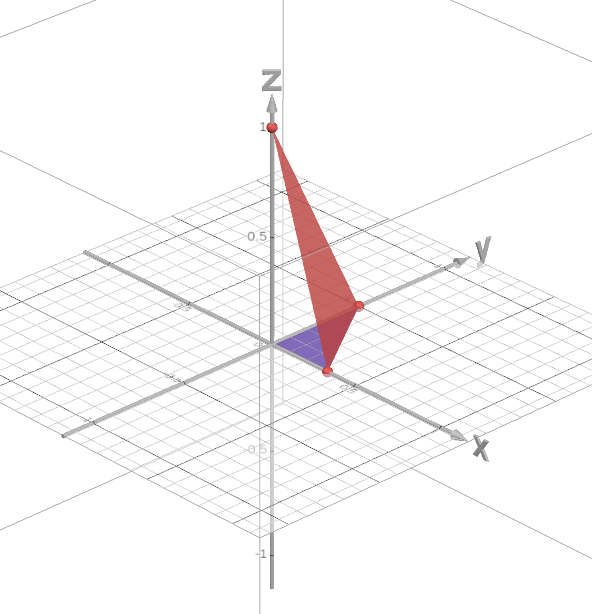
\includegraphics[scale=0.3]{problem8-16-9.png} \quad \quad 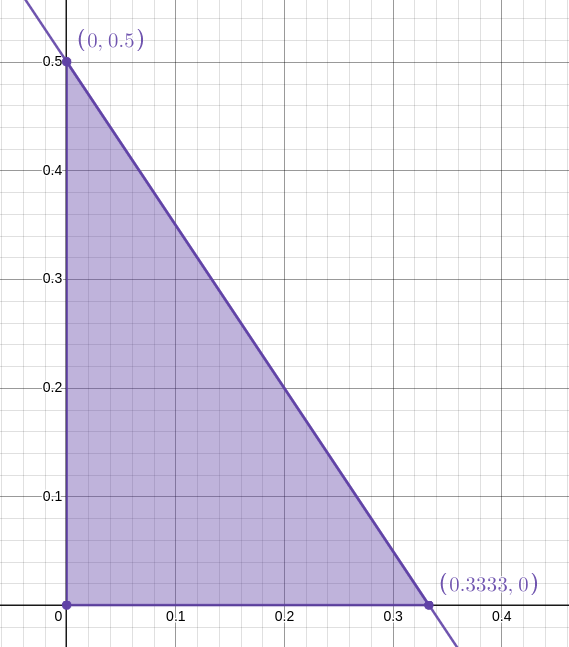
\includegraphics[scale=0.275]{problem8-16-9-RegionD.png}
	\end{center} 

	Since the curve is oriented counterclockwise as seen from above, using the ``Rule of Thumb'', the surface $S$ is oriented positively.	Let $\vec{r} (x, y) = \left\langle x , y , 1 - 3x - 2y \right\rangle$, so that $\vec{r}_x \times \vec{r}_y = \left\langle 3, 2, 1 \right\rangle$, with 
		$$
			D = \{ (x, y) \, : \, 0 \leq x \leq 1/3 , \, 0 \leq y \leq 1/2 - 3x/2 \} .
		$$ 
	Therefore, from Stokes' Theorem,
		\[
			\int_C \vec{F} \cdot d\vec{r} = \iint_S \curl \vec{F} \cdot d \vec{S} .
		\]
	We have
		\[
			\curl \vec{F} = \left\langle x - y , -y, 1 \right\rangle 
		\]
	and therefore
		\begin{align*}
			\int_C \vec{F} \cdot d \vec{r} &= \int_0^{1/3} \int_0^{1/2 - 3x/2} \left\langle x - y , -y , 1 \right\rangle \cdot \left\langle 3, 2, 1 \right\rangle \, dy dx \\ 
			&= \int_0^{1/3} \int_0^{1/2 - 3x/2} 3x - 5y + 1 \, dy dx = \fbox{$\displaystyle\frac{1}{24}$} .
		\end{align*}

	\spc 

	\exo{16.8}{12a \& 12b}{15}
	\begin{enumerate}[label=\alph*)]
	\item We will use the surface $S$ represented in the figure below. Also, the curve $C$ is pictured in purple.
		\begin{center}
		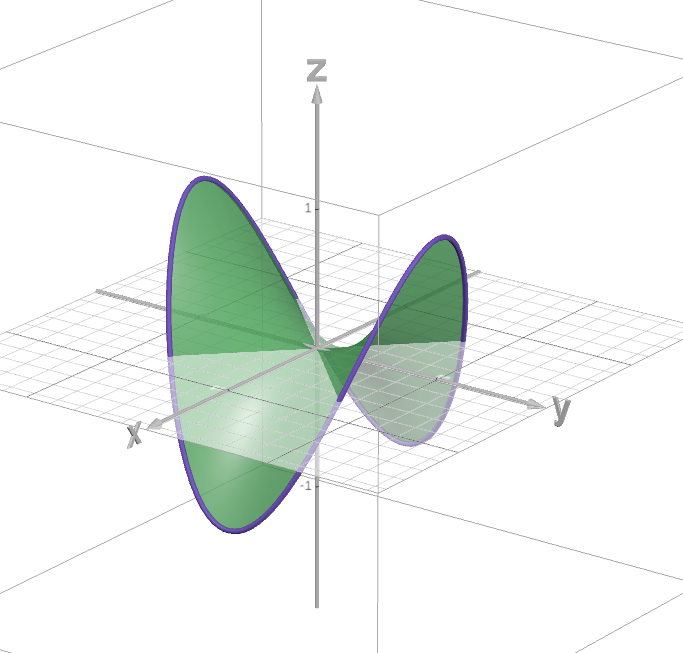
\includegraphics[scale=0.3]{problem12-16-9.png}
		\end{center}
	Using polar coordinates to parametrize the region $D$ inside the cylinder, we get
		\[
			\vec{r} (u, v ) = \left\langle u \cos v , u \sin v , u^2 \sin^2 (v) - u^2 \cos^2 (v) \right\rangle 
		\]
	with $D = \{ (u, v ) \, : \, 0 \leq u \leq 1 , 0 \leq v \leq 2 \pi \}$. Using Stokes' Theorem,
		\[
			\int_C \vec{F} \cdot d\vec{r} = \iint_S \curl \vec{F} \cdot d \vec{S} .
		\]
	Now, we have $2u^2 \sin (v) \cos^2 (v) + 2u^2 \sin^3 (v) $
		\[
			\vec{r}_u \times \vec{r}_v = \begin{vmatrix} \vec{i} & \vec{j} & \vec{k} \\ 
			\cos v & \sin v & 2u \sin^2 (v) - 2u\cos^2 (v) ) \\ 
			-u \sin v & u \cos v & 4u^2 \sin (v) \cos (v) \\ \end{vmatrix} = \left\langle 2u^2 \cos (v) , -2u^2 \sin (v) , u \right\rangle
		\]
	We see that the second component $-2u^2 \sin (v)$ of $\vec{r}_u \times \vec{r}_v$ can be rewritten as $-2u y$, where $y = u \sin (v)$ is the second component of the position vector $\vec{r}$ of $S$. Since $2u$ is always positive, the vector $\vec{r}_u \times \vec{r}_v$ will always point in opposite direction of the $y$ axis, given us the upward orentation. 

	Also, we compute
		\[
			\curl \vec{F} = \begin{vmatrix} \vec{i} & \vec{j} & \vec{k} \\ \frac{\partial}{\partial x} & \frac{\partial}{\partial y} & \frac{\partial}{\partial z} \\ x^2 y & (1/3) x^3 & xy \end{vmatrix} = \left\langle x , -y , 0 \right\rangle 
		\]
	Hence,
		\begin{align*}
			\iint_S \curl \vec{F} \cdot d \vec{S} &= \iint_D \left\langle u \cos v , -u \sin v , 0 \right\rangle \cdot \left\langle 2u^2 \cos (v) , - 2 u^2 \sin (v) , u \right\rangle \, dA \\ 
			&= \int_0^{2\pi} \int_0^1 2u^3 \cos^2 (v) + 2u^3 \sin^2 (v) \, du dv \\ 
			&= \int_0^{2\pi} \int_0^1 2u^3 \, du dv \\ 
			&= (2\pi ) (1/2 ) = \fbox{$\pi$} .
		\end{align*}
	\item See the picture in part (a) or the picture below:
		\begin{center}
		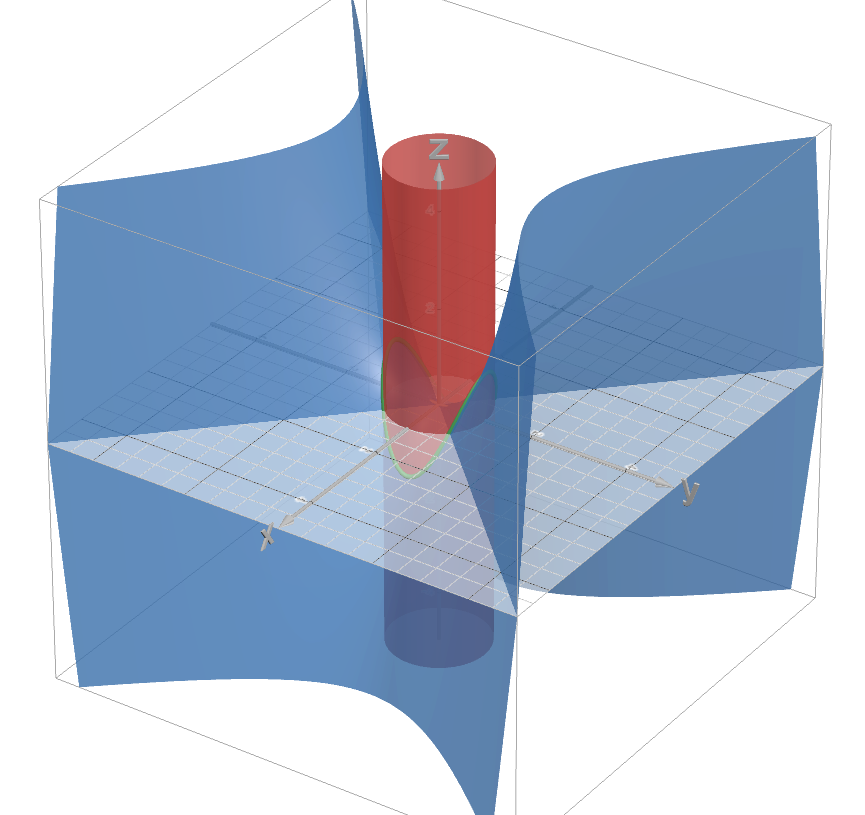
\includegraphics[scale=0.3]{picture12b.png}
		\end{center}
	\end{enumerate}

	\spc 

	\exo{16.8}{18}{10}
	\\ 
	Let $S$ be the part of the surface $z = 2xy$ that is inside the curve $C$. We can parametrize $S$ in the following way:
		\[
			\vec{r} (x, y) = \left\langle x , y, 2xy \right\rangle 
		\]
	with $D = \{ (x , y) \, : \, x^2 + y^2 \leq 1 \}$. Let 
		\[
			\vec{F} (x, y, z) = \left\langle P , Q , R \right\rangle = \left\langle y + \sin x , z^2 + \cos y , x^3 \right\rangle .
		\]
	Using Stokes' Theorem, we can write
		\[
			\int_C P dx + Q dy + R dz = \int_C \vec{F} \cdot d \vec{r} = \iint_S \curl \vec{F} \cdot d \vec{S} .
		\]
	We compute
		\[
			\vec{r}_x \times \vec{r}_y = \begin{vmatrix} \vec{i} & \vec{j} & \vec{k} \\ 1 & 0 & 2y \\ 0 & 1 & 2x \end{vmatrix} = \left\langle -2y, -2x, 1 \right\rangle 
		\]
	and
		\[
			\curl \vec{F} = \begin{vmatrix} \vec{i} & \vec{j} & \vec{k} \\ \frac{\partial}{\partial x} & \frac{\partial}{\partial y} & \frac{\partial}{\partial z} \\ y + \sin x & z^2 + \cos y & x^3 \end{vmatrix} = \left\langle -2z , -3x^2 , 1 \right\rangle .
		\]
	Since the $z$ component is positive, the vector $\vec{r}_x \times \vec{r}_y$ points upwards. However, the curve is oriented negatively and we should use $-\vec{r}_x \times \vec{r}_y$. Therefore,
		\begin{align*}
			\iint_S \curl \vec{F} \cdot d \vec{S} &= \iint_D \left\langle -4xy , -3x^2 , -1 \right\rangle \cdot \left\langle 2y , 2x , -1 \right\rangle \, dA \\ 
			&= \iint_D -8xy^2 + -6 x^3 + 1 \, dA \\ 
			\end{align*}
	Notice that if $f(x, y) = 8xy^2$, then $f(-x , y) = -8xy^2 = -f(x, y)$ and $f(x, -y) = f(x, y)$. Since $D$ is symmetric about the $x$-axis and the $y$-axis, we obtain
		\[
			\iint_D 8xy^2 = 0 .
		\]
	Using a similar argument with $g(x, y) = x^3$, we obtain
		\[
			\iint_D 6x^3 = 0 .
		\]
	Therefore,
		\[
			\iint_S \curl \vec{F} \cdot d\vec{S} = \iint_D 1 \, dA = \mathrm{Area} \, (D) = \pi .
		\]

\end{document}